% !TEX root =  ../Report.tex
\section{Figures, tables, algorithms}
\label{sec: figs tables algos}

The researcher and the supervisor both attended a photography for the new hill valley clock tower. This can be seen in figure \ref{fig:clock tower photo}.

\begin{figure}[h!]
    \centering
    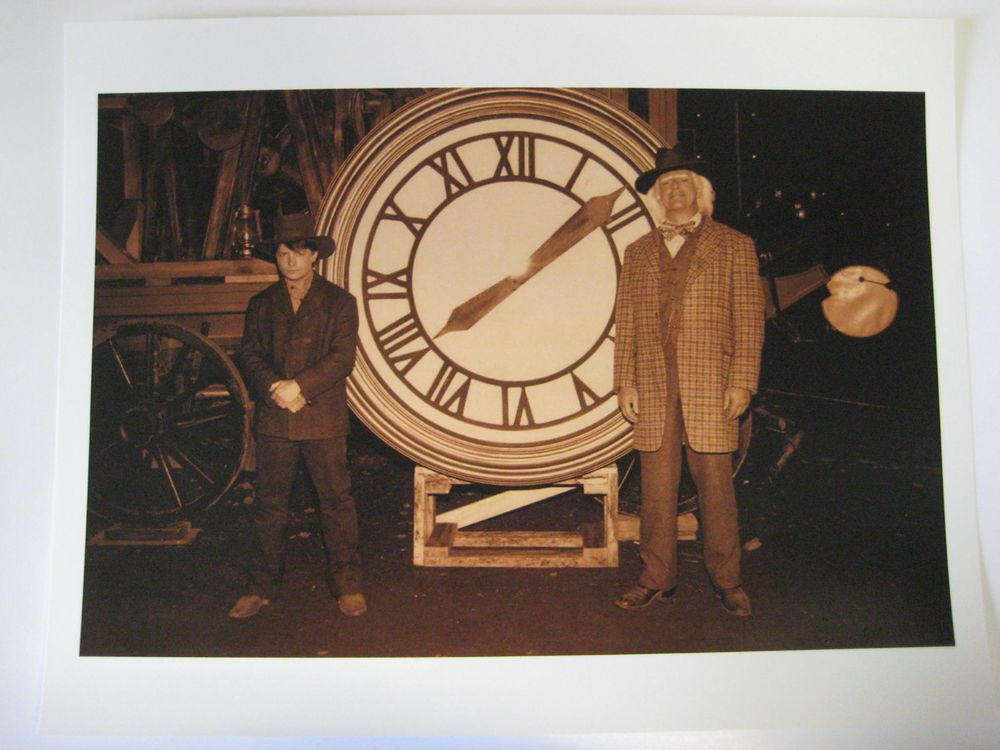
\includegraphics[width=\textwidth]{OriginalTemplate/Chapter2/doc_and_marty.jpg}
    \caption{The Researcher and Supervisor}
    \label{fig:clock tower photo}
\end{figure}

\noindent Again from figure \ref{fig:clock tower photo} we can see the researcher on the \textit{left} and the supervisor on the \textit{right}.\\

From this, a table was made for some of the items needed for temporal experiment number one to undergo completion. This is set to occur on \texttt{October 26, 1985, 1:18 A.M}.

\begin{table}[H] 
\begin{tabularx}{\textwidth}{| X | X |}
    \hline
     Item & Description  \\ \hline
     2 x Pocket Clocks & For measurement in time difference of machine and present time \\ \hline
     Einstein & The Dog test pilot \\ \hline
     JVC GR-C1 & VHS Camcorder \\ \hline
\end{tabularx}
\caption{Inventory list for temporal experiment number one}
\label{table: inventory}
\end{table}
